\documentclass{article}
\usepackage{spconf,amsmath,amssymb,graphicx,booktabs,microtype}
% hidelinks: the review PDF should carry no coloured frames around citations
% and URLs, which is what plain hyperref draws.
\usepackage[hidelinks]{hyperref}

\makeatletter
% spconf restyles only numbered headings: it redefines \@sect and leaves
% \@ssect alone, so \section* keeps article's much larger default and the
% unnumbered statement below would tower over the headings around it.
\def\@ssect#1#2#3#4#5{%
  \begingroup\bf\centering
  {\interlinepenalty \@M \uppercase{#5}\par}%
  \endgroup
  \@tempskipa #3\relax
  \@xsect{\@tempskipa}}
\makeatother

\title{TARGET-DATA ACCESS AND AGGREGATION EFFECTS IN CROSS-SUBJECT EEG EVALUATION}

\name{Chenghao Li$^{\star}$ \qquad Haochen Zhou$^{\dagger}$ \qquad Chunfeng Yang$^{\ddagger}$}
\address{%
$^{\star}$College of Software Engineering, Southeast University, Nanjing, China \\
$^{\dagger}$School of Artificial Intelligence, Southeast University, Nanjing, China \\
$^{\ddagger}$School of Computer Science and Engineering, Southeast University, Nanjing, China \\
\texttt{\{yo666666yo, 213241737, chunfeng.yang\}@seu.edu.cn}}

\begin{document}
\ninept
\maketitle

\begin{abstract}
Cross-subject EEG decoders are compared across protocols that use the target subject differently, and the gaps between them are read as the value of that access. That reading holds only if everything else is matched. We divide each held-out subject's trials into an available half and a reserved half, score every condition on the same reserved half, and cross two procedures: Euclidean Alignment and supervised training on the available half. The source partition, epoch budget, target sampling rate and scored trials are fixed and checked against the realized indices. On three motor-imagery datasets spanning 9 to 105 subjects both procedures help, but their ordering reverses and no interaction replicates; capping the calibration set rules out its size as the cause. A second control, regrouping identical predictions without retraining, shows a reported between-subject spread also tracks the trials per subject. Neither what target access buys nor what a spread means is portable across datasets.
\end{abstract}

\begin{keywords}
Brain--computer interfaces, cross-subject evaluation, Euclidean alignment, calibration data, between-subject variability
\end{keywords}

\section{Introduction}

Cross-subject EEG decoders are compared across papers whose evaluation protocols use the target subject differently. Some use none of it, some use its unlabelled signals to align feature distributions, some fine-tune on a labelled calibration block. The labels attached to these protocols---zero-calibration, unsupervised transfer, subject-adaptive---are coarse, and the accuracy differences between them are routinely read as the value of the extra access.

That reading requires the comparison to hold everything else constant, and published comparisons rarely can. Adding a calibration block lengthens an epoch, so the adapted model also gets more optimizer steps; the target's share of a batch is whatever the cohort size implies; and if the block supplies the early-stopping signal, model selection has changed too. None of this is visible in a results table, and all of it moves with the effect being claimed. Our own earlier work tracked those quantities rather than the procedure; Section~\ref{sec:controls} reports what replaying it shows.

This paper asks a narrower question that can be answered cleanly. \textbf{On a fixed target test set, what does each way of using the target subject's available trials buy, once the source partition, the per-epoch sample budget, the early-stopping rule and the target sampling rate are held constant?} Each held-out subject's trials are divided once into an available half and a reserved test half, and every condition is scored on the same reserved half. The available half is used in one of four ways: not at all, by Euclidean Alignment, by supervised training, or by both. This crosses two \emph{procedures}, not two independent kinds of access---supervised training reads the available trials' signals as well as their labels---so the grid separates what each procedure adds on top of the other, not the value of signals against labels.

\textbf{Related work.} Partitioning and reporting choices are known to move BCI comparisons \cite{lotte2018review,roy2019deep}, and MOABB standardizes the interface but not the accounting \cite{jayaram2018moabb}: two pipelines can share a loader and a split while giving the target subject different influence over training, normalization and checkpoint choice. Euclidean Alignment reads the evaluated subject's trials but none of their labels and is routinely called zero-calibration \cite{he2020transfer}, while calibration-block fine-tuning consumes labels outright; compact convolutional references \cite{lawhern2018eegnet,schirrmeister2017deep} carry both. Leakage drives irreproducible findings \cite{kapoor2023leakage} and small-sample neuroimaging yields error bars wider than reported \cite{varoquaux2018crossval}, but that work is diagnostic, whereas choosing between protocols needs what a procedure is worth once everything else is matched.

A second question concerns how the result is summarized. A cross-subject paper reports a spread as well as a mean, and the spread is read as between-subject heterogeneity. That holds only if the aggregation unit is the subject. We test it with a control that retrains nothing: the same per-trial predictions are aggregated by true subject and by random groups of the same sizes, so any difference is attributable to the grouping alone.

\textbf{Contributions.} (i) A controlled $2\times2$ of alignment against target supervision on three motor-imagery datasets spanning 9 to 105 subjects, with the source partition, the epoch and the scored trials pinned and checked against the realized indices, and with the exposure quantities that \emph{cannot} simultaneously be pinned reported instead. (ii) A fixed-prediction regrouping benchmark, and a matching variance estimate, for how much of a reported between-subject spread the aggregation unit accounts for. (iii) An audit of what an uncontrolled version of the same comparison reports instead. Code, logs and per-trial predictions: \url{https://github.com/yo666666yo/target-data-access-eeg}. The split, the resampling and alignment itself are standard; what is new is the set of controls under which the comparison is made, and the account of which cannot hold at once.

% Related work is folded into the introduction to fit the four-page limit.
% sections/015_related.tex is retained for the longer arXiv version.
%\section{Related Work}
\label{sec:related}

Partitioning, preprocessing and reporting choices have long been known to move BCI comparisons \cite{lotte2018review,roy2019deep}, and the MOABB ecosystem was built to make evaluation uniform across pipelines \cite{jayaram2018moabb}. Standardization constrains the interface rather than the accounting: two pipelines can consume the same loader and the same split specification while giving the target subject different amounts of influence over training, normalization and checkpoint choice.

Euclidean Alignment is the standard remedy for inter-subject covariate shift in motor imagery \cite{he2020transfer}; it reads the evaluated subject's trials but none of their labels, and results using it are routinely described as zero-calibration. Calibration-block fine-tuning sits at the other end and consumes labels outright. Compact convolutional references such as EEGNet \cite{lawhern2018eegnet} and its relatives \cite{schirrmeister2017deep} carry both. What is rarely reported is how much of the difference between two such pipelines is the procedure, and how much is the training budget, the batch composition or the selection signal that moved alongside it.

Leakage is a recognized driver of irreproducible findings \cite{kapoor2023leakage}, and small-sample neuroimaging evaluation produces error bars wider than reported \cite{varoquaux2018crossval}. That work is largely diagnostic: it establishes that a pipeline leaks and an estimate is inflated. Choosing between protocols also requires knowing what a procedure is worth once everything else is matched. Relatedly, a cross-subject spread is read as between-subject heterogeneity, but that depends on the aggregation unit and the trials each unit holds: with 45 test trials per subject, finite-sample noise alone yields a spread of several accuracy points. That trial-wise and subject-wise groupings answer different questions is established; what we add is a measurement of the gap, from predictions held fixed.

We contribute no architecture and claim no state of the art. The contribution is a measurement design: a $2\times2$ of alignment against target supervision with the source partition, optimizer budget, target sampling rate and scored trials pinned and checked against the realized indices, on the official BCI Competition IV 2a release \cite{tangermann2012bcicompiv} and two further motor-imagery datasets, with subject-paired intervals and a fixed-prediction control for the aggregation unit.

\section{Method}
\label{sec:method}

\begin{figure*}[t]
    \centering
    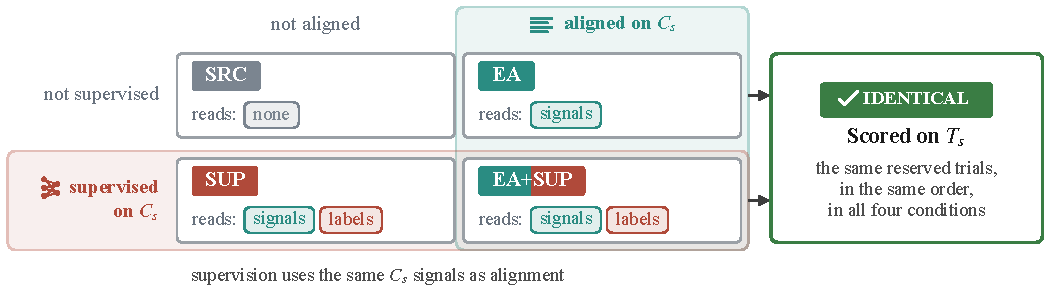
\includegraphics[width=\textwidth]{figures/figure2.pdf}
    \caption{The four conditions as a $2\times2$ over the two procedures, with what each reads from the held-out subject's available half $C_s$. Supervised training reads those trials' signals as well as their labels, so the procedures overlap. Everything else is held fixed, as Section~\ref{sec:controls} sets out, and all four are scored on the same reserved trials in the same order.}
    \label{fig:grid}
\end{figure*}

\subsection{Conditions}
We evaluate leave-one-subject-out on the three motor-imagery datasets of Table~\ref{tab:datasets}. Each held-out subject's trials are divided once, stratified by class under a per-subject seed, into an available half $C_s$ and a reserved half $T_s$ (Fig.~\ref{fig:overview}b); that 50/50 division is the declared target-data budget, no condition can change it, and $T_s$ is only ever scored.

Figure~\ref{fig:grid} shows the design. Both procedures read $C_s$: supervised training on it consumes those trials' signals as well as their labels. Each axis of the grid names a procedure applied to those trials, and both axes have the same access to them.

Alignment uses signals and no labels. Euclidean Alignment~\cite{he2020transfer} whitens a subject's trials by $\bar{R}^{-1/2}$, where $\bar{R}$ is the mean over that subject's trials of the sample spatial covariance $XX^{\top}/T$, computed on the band-passed epochs with no shrinkage and inverted through an eigendecomposition whose eigenvalues are floored at $10^{-10}$ to keep a rank-deficient epoch from blowing up. Source subjects are whitened by a reference estimated from all of their trials, which is legitimate because all of them are available. The held-out subject's reference is estimated from $C_s$ alone and then frozen; $T_s$ is transformed by it but never contributes to it. The switch also changes how every source subject is preprocessed, so the measured effect is that of the whole alignment pipeline. Target supervision adds $C_s$ to the training set with its labels attached.

The four conditions are neither procedure (SRC), alignment only (EA), supervision only (SUP), and both (EA+SUP). Two further arms sit off the grid, each changing a third thing: SEL picks the checkpoint on $C_s$ rather than the source validation set, leaving training set, initialization and trajectory unchanged but swapping a selection set of very different size; POOL adds $C_s$ to the same scaler's fit set. $T_s$ enters no scaler.

\begin{table}[b]
\centering
\caption{The three motor-imagery datasets. Trials per half is the declared target-data budget: each held-out subject is cut once into an available half $C_s$ and a reserved test half $T_s$ of that size. Chance is given in parentheses; it differs across the datasets, so accuracies are not comparable between them.}
\label{tab:datasets}
\small
\setlength{\tabcolsep}{4pt}
\begin{tabular}{@{}lcccc@{}}
\toprule
& Subjects & Channels & Classes & Trials/half \\
\midrule
BCI IV 2a \cite{tangermann2012bcicompiv} & 9 & 22 & 4 ($0.25$) & 288 \\
BNCI2014-002 \cite{steyrl2016bnci} & 14 & 15 & 2 ($0.50$) & 80 \\
PhysionetMI \cite{schalk2004bci2000,goldberger2000physionet} & 105 & 64 & 4 ($0.25$) & 45 \\
\bottomrule
\end{tabular}
\end{table}


\subsection{Controlled variables}
\label{sec:controls}
Three quantities are pinned exactly:
\begin{itemize}[nosep,leftmargin=1.2em]
\item the source partition: the stratified 80/20 split supplying training and selection data is derived from the outer pool alone and is the same index set in all four conditions, and validation is source-only throughout, so target trials never reach the selection set;
\item the epoch: every condition draws, with replacement, as many samples per epoch as the source training set holds (3686, 1664 and 7486);
\item the scored object: $T_s$ is identical across conditions, trial for trial.
\end{itemize}
A fourth, the target sampling rate, is fixed in expectation: a plain shuffled loader over the same pool would give the target 7.2\%, 4.6\% and 0.6\% of a batch, a 12-fold range set by cohort size. The supervised arms therefore use a weighted sampler with a declared expected share of 0.10, realized at 0.096--0.109.

Two quantities this does not equalize, and we report both. Because the epoch is a fixed total, a supervised arm draws 10\% fewer source samples per epoch than SRC; and because each arm early-stops on its own curve, realized updates differ: taking fold-averaged totals per arm and dividing the spread by the smallest, by 10\% on 2a, 3\% on PhysionetMI and 23\% on BNCI2014-002. Exposure is the sharper problem: a declared share $w$ implies $wS/|C_s|$ expected draws of each target trial per epoch, which is 1.3, 2.1 and 16.6 here, since $|C_s|$ differs 6.4-fold. Matching repetition instead would need shares of 0.156, 0.096 and 0.012; matching both would need source exposure to vary 13-fold. Any such comparison fixes two of these three and lets the third move, which is why we vary $|C_s|$ directly in Section~\ref{sec:results}.

An earlier version of this study enforced none of these controls, and replaying it gives the pattern of Fig.~\ref{fig:overview}a: a supervised arm on a re-drawn source partition with target trials in its validation set and batch shares of 6.1, 3.8 and 0.5\%, which its cross-dataset ordering followed; a selection arm with 25\% more source trials than its reference; and a whitener fitted on $C_s \cup T_s$. None shows in a results table, so a script checks the controls against the realized indices before any run.

\subsection{Aggregation unit}
\label{sec:aggregation}
A cross-subject spread is read as between-subject heterogeneity, which requires the aggregation unit to be the subject. We test that with a control that retrains nothing: the per-trial predictions on $T_s$ are held fixed and only the grouping changes, first by true subject, then into random groups of the same sizes, 2000 times, on SRC and SUP. Trial-weighted accuracy is identical either way, and subjects contribute equal trial counts on 2a and BNCI2014-002 and near-equal ones on PhysionetMI (45 for 104 subjects, 44 for one), so the subject macro-average and the trial-weighted average coincide up to that single trial and any difference in spread belongs to the grouping alone. The null is not a new phenomenon: drawing $m$ of $M$ correctness records without replacement gives group means of variance $(1-m/M)S^2/m$, which our resampled null reproduces. What it adds is how much of a reported spread that accounts for, where $m$ ranges from 45 to 288.

\subsection{Statistics}
\label{sec:stats}
Each subject contributes one number per condition, averaged over three runs. Those runs vary the target split and the initialization together, so they estimate neither alone; within a run all conditions share both, which is what the pairing requires. Differences are paired within subject and resampled over subjects, with one set of bootstrap indices drawn per dataset and reused for every condition ($10^4$ replicates, percentile intervals~\cite{efron1994bootstrap}). $p$-values come from a two-sided sign-flip permutation test~\cite{winkler2014permutation} over the five conditions of a dataset, Holm-corrected~\cite{holm1979simple} within that family, with a paired $t$-test as a sensitivity check. That test saturates on a small cohort: on nine subjects it cannot return less than $2/2^{9}=0.0039$, so we report the number of subjects helped beside it. Spread comparisons are ratios of standard deviations, so every factor quoted below is on that scale.

Because leave-one-subject-out folds share most of their training pool, the subjects are not independent replicates~\cite{nadeau2003inference}, and with nine of them on 2a the reference distribution is coarse. We therefore read a Holm-adjusted $p$ below 0.05 as a difference resolved by this repetition structure (these subjects, these runs, this training policy) and not as inference about a subject population, and we use that as the single rule for which differences we state. Intervals give magnitude only: they carry no multiplicity adjustment, and in a Gaussian simulation at $n=9$ our percentile intervals covered 89\% rather than 95\%, so an interval excluding zero beside a non-significant adjusted $p$ is not evidence of an effect.

\section{Results}
\label{sec:results}

\subsection{Setup}
BCI Competition IV 2a \cite{tangermann2012bcicompiv} is read from the competition archives, band-passed 8--32\,Hz over the four seconds after the cue, with EOG dropped by the official channel contract and sessions T and E concatenated in that order. BNCI2014-002 \cite{steyrl2016bnci} is right hand versus feet. PhysionetMI \cite{schalk2004bci2000,goldberger2000physionet} drops its rest class, and subjects 88, 89, 92 and 100 are excluded for non-standard sampling. The latter two are loaded through MOABB \cite{jayaram2018moabb} with its motor-imagery paradigm at its default 8--32\,Hz, each over its own declared trial interval.

The decoder is our own reimplementation of EEGNet \cite{lawhern2018eegnet}, with $F_1=8$ temporal filters, depth multiplier $D=2$, $F_2=16$ pointwise filters and a temporal kernel of 64 samples. It omits the max-norm constraints of the original, one of which braindecode's implementation~\cite{schirrmeister2017deep} applies, so Section~\ref{sec:reference} repeats the whole grid with that decoder swapped in. Training uses Adam~\cite{kingma2015adam} ($10^{-3}$, weight decay $10^{-4}$), batch 64, $\leq50$ epochs, step decay ($\times0.5$ every 15) with patience 10 and class-balanced loss, with features standardized by one scaler fitted on source training trials.

\subsection{Condition effects}
Table~\ref{tab:main} gives the source-only references and the effects. Chance differs across the three datasets, so the reference accuracies are not comparable to one another; every claim below is a within-subject difference against an arm's own reference. Supervision rejects on all three datasets and alignment on two of three, with effect sizes that do not transfer across them, and the ordering between the two reverses.

\begin{table*}[t]
\centering
\caption{Effect of each procedure against the source-only reference under the controls of Section~\ref{sec:controls}. Differences are paired within subject and averaged over three runs; the per-run column gives the same difference within each run. Intervals are descriptive percentile bootstrap over subjects, not multiplicity-adjusted; $p$ is Holm-corrected within each dataset and is followed by the number of subjects helped, which distinguishes arms at the permutation floor. SD is the between-subject standard deviation of run-averaged per-subject accuracy---a different pooling order from Section~\ref{sec:results}, which pools variances within runs. \textsc{sel} and \textsc{pool} sit off the grid and are quoted in the text.}
\label{tab:main}
\small
\begin{tabular}{llccccc}
\toprule
Condition & Uses $C_s$ to & $\Delta$ accuracy (pp) [95\% CI] & per run (pp) & subject SD & SD ratio [95\% CI] & $p$ (improved) \\
\midrule
\multicolumn{7}{l}{\textit{BCI IV 2a} ($n=9$ subjects; source-only accuracy $0.450$, between-subject SD $0.175$)} \\
\textsc{ea} & align & $+1.58$ [$+0.17$, $+2.98$] & $+0.7$ $+2.1$ $+1.9$ & $0.180$ & $1.03$ [$0.94$, $1.13$] & 0.176 (7/9) \\
\textsc{sup} & supervise & $+9.45$ [$+5.88$, $+12.81$] & $+9.0$ $+9.1$ $+10.3$ & $0.196$ & $1.12$ [$0.88$, $1.36$] & 0.019 (9/9) \\
\textsc{ea+sup} & align + supervise & $+13.66$ [$+9.53$, $+17.44$] & $+12.2$ $+13.5$ $+15.3$ & $0.199$ & $1.14$ [$0.84$, $1.36$] & 0.019 (9/9) \\
\midrule
\multicolumn{7}{l}{\textit{BNCI2014-002} ($n=14$ subjects; source-only accuracy $0.687$, between-subject SD $0.115$)} \\
\textsc{ea} & align & $+8.07$ [$+4.37$, $+11.96$] & $+6.3$ $+7.5$ $+10.4$ & $0.120$ & $1.04$ [$0.78$, $1.49$] & 0.005 (12/14) \\
\textsc{sup} & supervise & $+6.52$ [$+3.18$, $+10.27$] & $+5.9$ $+3.8$ $+9.8$ & $0.136$ & $1.18$ [$0.95$, $1.64$] & 0.005 (12/14) \\
\textsc{ea+sup} & align + supervise & $+11.13$ [$+6.34$, $+16.16$] & $+10.8$ $+10.4$ $+12.2$ & $0.118$ & $1.02$ [$0.68$, $1.59$] & 0.002 (13/14) \\
\midrule
\multicolumn{7}{l}{\textit{PhysionetMI} ($n=105$ subjects; source-only accuracy $0.444$, between-subject SD $0.124$)} \\
\textsc{ea} & align & $+9.12$ [$+7.40$, $+10.81$] & $+10.9$ $+7.0$ $+9.5$ & $0.151$ & $1.22$ [$1.09$, $1.37$] & $<$0.001 (93/105) \\
\textsc{sup} & supervise & $+4.89$ [$+3.41$, $+6.41$] & $+5.5$ $+3.7$ $+5.5$ & $0.159$ & $1.28$ [$1.16$, $1.42$] & $<$0.001 (72/105) \\
\textsc{ea+sup} & align + supervise & $+12.68$ [$+11.04$, $+14.35$] & $+13.9$ $+10.5$ $+13.7$ & $0.159$ & $1.28$ [$1.16$, $1.43$] & $<$0.001 (99/105) \\
\bottomrule
\end{tabular}
\end{table*}


Alignment is worth $+1.58$ percentage points (pp) on 2a, where it does not survive correction (7 of 9 subjects, Holm $p=0.18$), against $+8.07$ and $+9.12$\,pp on BNCI2014-002 and PhysionetMI, where it does (12/14 and 93/105, $p\le0.005$). Target supervision runs the other way: $+9.45$\,pp on 2a, helping every subject, falling to $+6.52$ and $+4.89$\,pp on the larger cohorts. Comparing the two directly is exploratory, prompted by this ordering rather than specified in advance. On that comparison supervision leads alignment by $+7.87$\,pp [$+4.95, +11.03$] on 2a, is indistinguishable from it on BNCI2014-002 ($-1.55$ [$-4.46, +0.89$]), and trails it by $-4.23$\,pp [$-5.84, -2.64$] on PhysionetMI. Both endpoints reject under the decision rule (Holm-adjusted within these three tests, $p=0.008$ and $p<0.001$), so the observed contrasts do not support a common ordering across datasets. Being exploratory, the reversal stands as an observation in these runs and awaits a pre-specified test.

The calibration budget is confounded with the dataset, $|C_s|$ differing 6.4-fold, so we re-ran the arms that consume it with $|C_s|$ capped by a nested stratified subset and $T_s$ untouched. Shrinking it moves the effect monotonically but only a little: at a common budget of 45 trials the three datasets read $+5.88$, $-2.62$ and $-4.23$\,pp, so the ordering holds and the budget accounts for only about 2 of the 12 pp separating 2a from PhysionetMI. Within 2a the lead of supervision falls from $+7.87$\,pp at 288 available trials to $+7.29$ at 144 and $+5.88$ at 45, as each trial goes from being drawn 1.3 times per epoch to 8.4; within BNCI2014-002 it moves from $-1.55$ to $-2.62$, and only at the smaller budget does it resolve ($p=0.049$ against $p=0.33$). Budget does move the contrast, and in the direction that shrinks it, but by less within a dataset than separates one dataset from another.

Whether the two procedures compose additively is undetermined. Write the interaction as the gain alignment contributes on top of supervision, less the gain it contributes on its own,
\begin{equation}
\label{eq:interaction}
\Delta_{\mathrm{int}} = (\mathrm{EA{+}SUP} - \mathrm{SUP}) - (\mathrm{EA} - \mathrm{SRC}).
\end{equation}
Its estimate is $+2.62$, $-3.45$ and $-1.33$\,pp on the three datasets, and none of the three is resolved under the decision rule of Section~\ref{sec:stats}. The sign of $\Delta_{\mathrm{int}}$ is consistent across runs within a dataset but not across datasets, so it may itself be dataset-dependent. We therefore report neither evidence for additivity nor evidence against it.

\subsection{Control checks}
\label{sec:reference}
Two things could make these effects artefacts of our setup rather than of the protocol. The random split interleaves the halves in time, so they share drift and attention state; BCI IV 2a's two sessions let the same 288/288 budget be partitioned chronologically, and over five runs the effects change little: the lead of supervision over alignment is $+7.75$\,pp [$+5.54$, $+10.29$] under the chronological partition against $+7.87$\,pp under the random one, which makes that contrast cross-session. And the decoder is our own reimplementation, so we repeated the grid with braindecode's EEGNetv4 (0.8.1, matched hyper-parameters) swapped in: source-only accuracy moves by $-0.81$, $+0.27$ and $-0.55$\,pp, so the low reference is not attributable to our implementation alone, and the reversal reproduces, at $+8.27$\,pp on 2a and $-4.65$\,pp on PhysionetMI. EA and SUP reproduce wherever they reject; SEL on BNCI2014-002 does not. These runs and the capped-budget ones carry their own source snapshots.

\subsection{Aggregation effects}
Holding the predictions fixed and changing only the grouping, the resampled null matches the finite-population prediction to within 0.0013 and tracks the trials per group, though it also depends on the pooled accuracy and the group count. With 288 test trials each on 2a it is 0.029 against 0.177 by true subject, a factor of 6.2, falling to 2.4 with 80 trials and 1.8 with 45; the supervised arm behaves likewise (6.99, 2.96, 2.23), though not at the same size, so the gap is not independent of training.

That null serves as a benchmark: shuffling removes the subject structure along with the trial noise, so it cannot decompose the spread. Estimating the two components separately instead, under a conditionally binomial model, puts finite trials at 2\%, 17\% and 29\% of the observed between-subject variance and leaves standard deviations of 0.174, 0.111 and 0.113 against raw values of 0.177, 0.122 and 0.134; the estimator, its assumptions and the per-run terms are in the repository. Raw figures rank PhysionetMI as the more heterogeneous cohort and corrected ones do not, though that gap is unresolved ($+0.002$ [$-0.031$, $+0.024$]). The control itself establishes only that spread exceeds the benchmark everywhere ($p < 0.001$).

\subsection{Off-grid arms}
Choosing the checkpoint on $C_s$ can cost accuracy: SEL is $-1.69$\,pp [$-2.80$, $-0.55$] on PhysionetMI, helping 37 of 105 subjects, surviving correction ($p=0.009$) and reproducing under the reference decoder ($-1.81$). That is where the selection set is smallest, 45 trials against the 1872 it replaces. Its positive values elsewhere do not reproduce, so we claim only this direction. No POOL arm rejects.

\section{Discussion}

Some readings these numbers do not support. The reference accuracies sit below those usually quoted, but standardization, budget, schedule, alignment and a reference decoder each failed to account for the gap, so the discrepancy cannot be attributed to our implementation alone. A large alignment gain is likewise no evidence of a violation: admissibility turns on whether the claimed deployment permits reading the target's unlabelled signals. Nor is the supervised effect the value of labels. A fixed batch share replays each PhysionetMI target trial 16.6 times per epoch against 1.3 on 2a, which made overfit to a small, repeatedly drawn $C_s$ a candidate explanation for the reversal; capping $|C_s|$ makes that explanation insufficient on its own. The remaining difference is dataset-dependent in these runs, but we do not resolve its cause further. SEL's harm is a separate route: it never trains on $C_s$, only picks a checkpoint there, so what is at stake is selection noise on 45 validation trials rather than training overfit, a distinction these runs do not resolve.

Limitations are two decoders, one alignment method, one sampling rate, and one 50/50 budget; the chronological split was available only on 2a. Section~\ref{sec:stats} states the decision rule and the intervals' limits.


% Permitted on the optional fifth page alongside references and funding notes.
\section*{Compliance with Ethical Standards}
This work is a secondary analysis of three public motor-imagery EEG corpora---BCI Competition IV
dataset 2a, BNCI2014-002 and the PhysioNet EEG Motor Movement/Imagery database---each released by
its originators for open research use with participant consent and ethical approval obtained by
the original investigators. No new data were recorded and no human participants were involved in
this study, so no additional ethical approval was required. The authors declare no conflict of
interest.

\bibliographystyle{IEEEbib}
\bibliography{references}
\end{document}
